\documentclass{report}
\usepackage[utf8]{inputenc}

%----- Configuración del estilo del documento------%
\usepackage{epsfig,graphicx}
\usepackage[left=2.5cm,right=2.5cm,top=1.8cm,bottom=2.3cm]{geometry}
%------ Paquetes matematicos --------%
\usepackage{amsmath}
\usepackage{amssymb}
\usepackage{amsthm}
\usepackage{amsmath}
\usepackage{tabularx}
\usepackage{fancyhdr}
\usepackage{lastpage}
\usepackage{verbatim}
\usepackage[shortlabels]{enumitem}
\usepackage{venndiagram}
\usetikzlibrary{shapes.geometric}
\usepackage{cancel}
\usepackage{hyperref}
\usepackage[T1]{fontenc}
\usepackage[spanish,es-nodecimaldot,es-tabla]{babel}
\usepackage{csquotes}
\usepackage{graphicx}
\usepackage{tocloft}
\graphicspath{{./figs/}}
\usepackage{setspace}
\usepackage{xcolor}


\usepackage[backend=biber]{biblatex}
\addbibresource{resources/referencias/referencias.bib}




\begin{document}
	
	\begin{titlepage}
	\thispagestyle{empty}
	\begin{minipage}[c][0.17\textheight][c]{0.25\textwidth}
		\begin{center}
			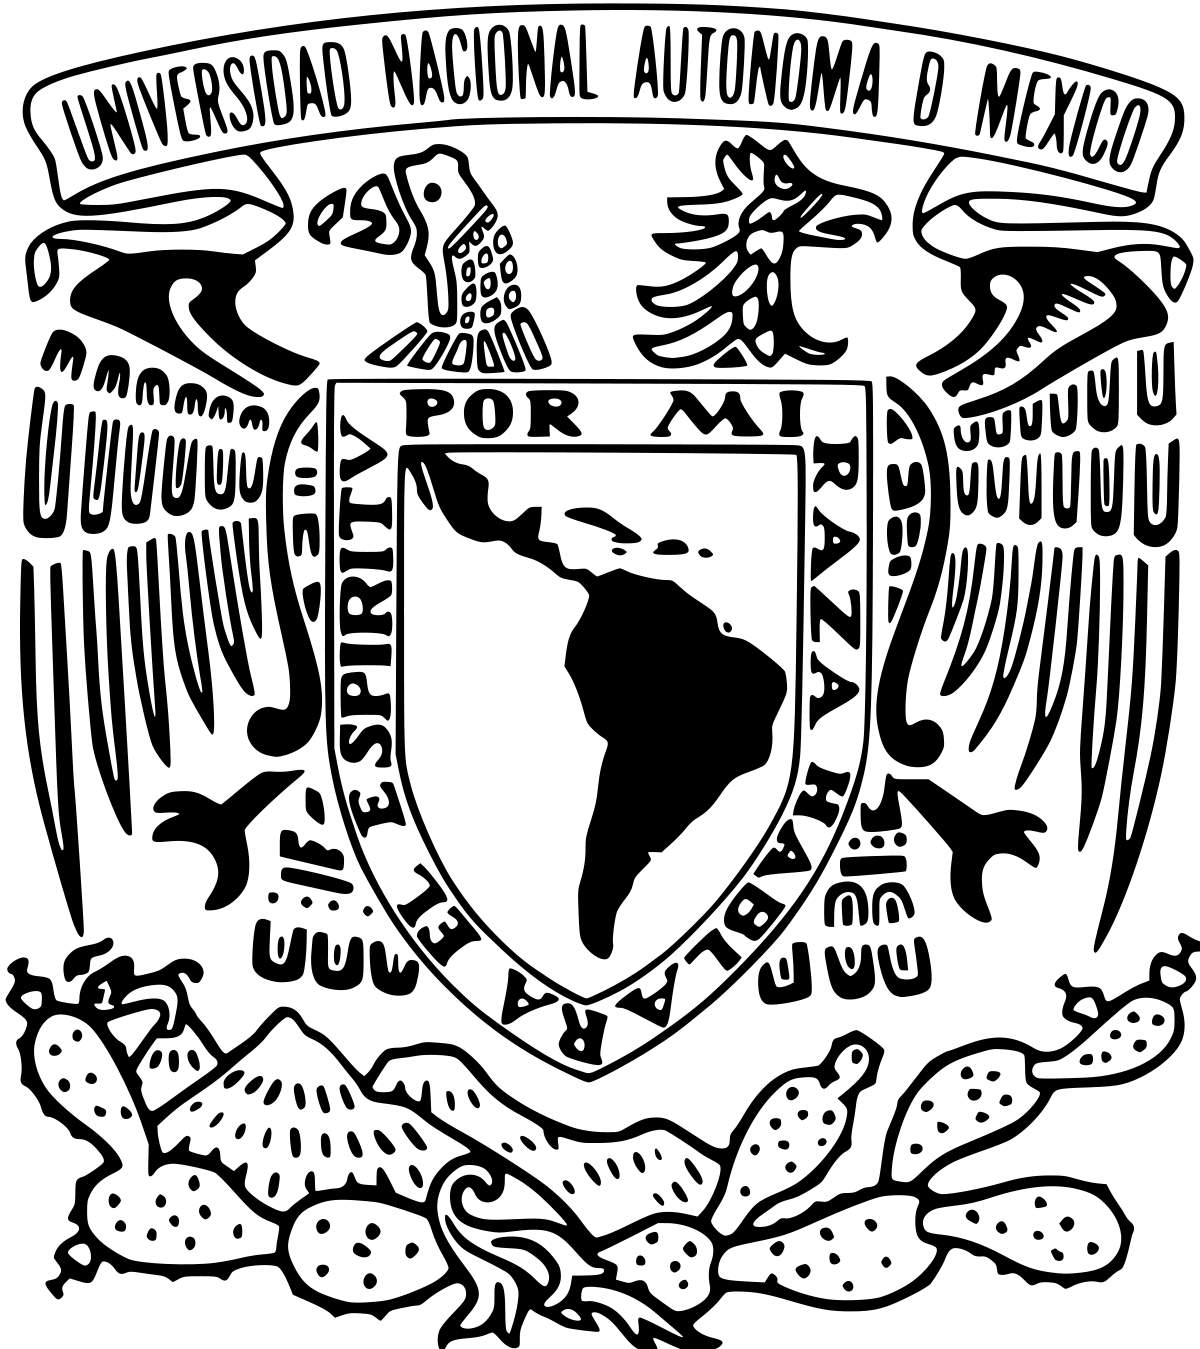
\includegraphics[width=3.5cm, height=3.5cm]{resources/Logo_UNAM.png}
		\end{center}
	\end{minipage}
	\begin{minipage}[c][0.195\textheight][t]{0.75\textwidth}
		\begin{center}
			\vspace{0.3cm}
			\textsc{\large Universidad Nacional Aut\'onoma de M\'exico}\\[0.5cm]
			\vspace{0.3cm}
			\hrule height2.5pt
			\vspace{.2cm}
			\hrule height1pt
			\vspace{.8cm}
			\textsc{Facultad de Ciencias}\\[0.5cm] %
		\end{center}
	\end{minipage}
	
	\begin{minipage}[c][0.81\textheight][t]{0.25\textwidth}
		\vspace*{5mm}
		\begin{center}
			\hskip2.0mm
			\vrule width1pt height13cm 
			\vspace{5mm}
			\hskip2pt
			\vrule width2.5pt height13cm
			\hskip2mm
			\vrule width1pt height13cm \\
			\vspace{5mm}
			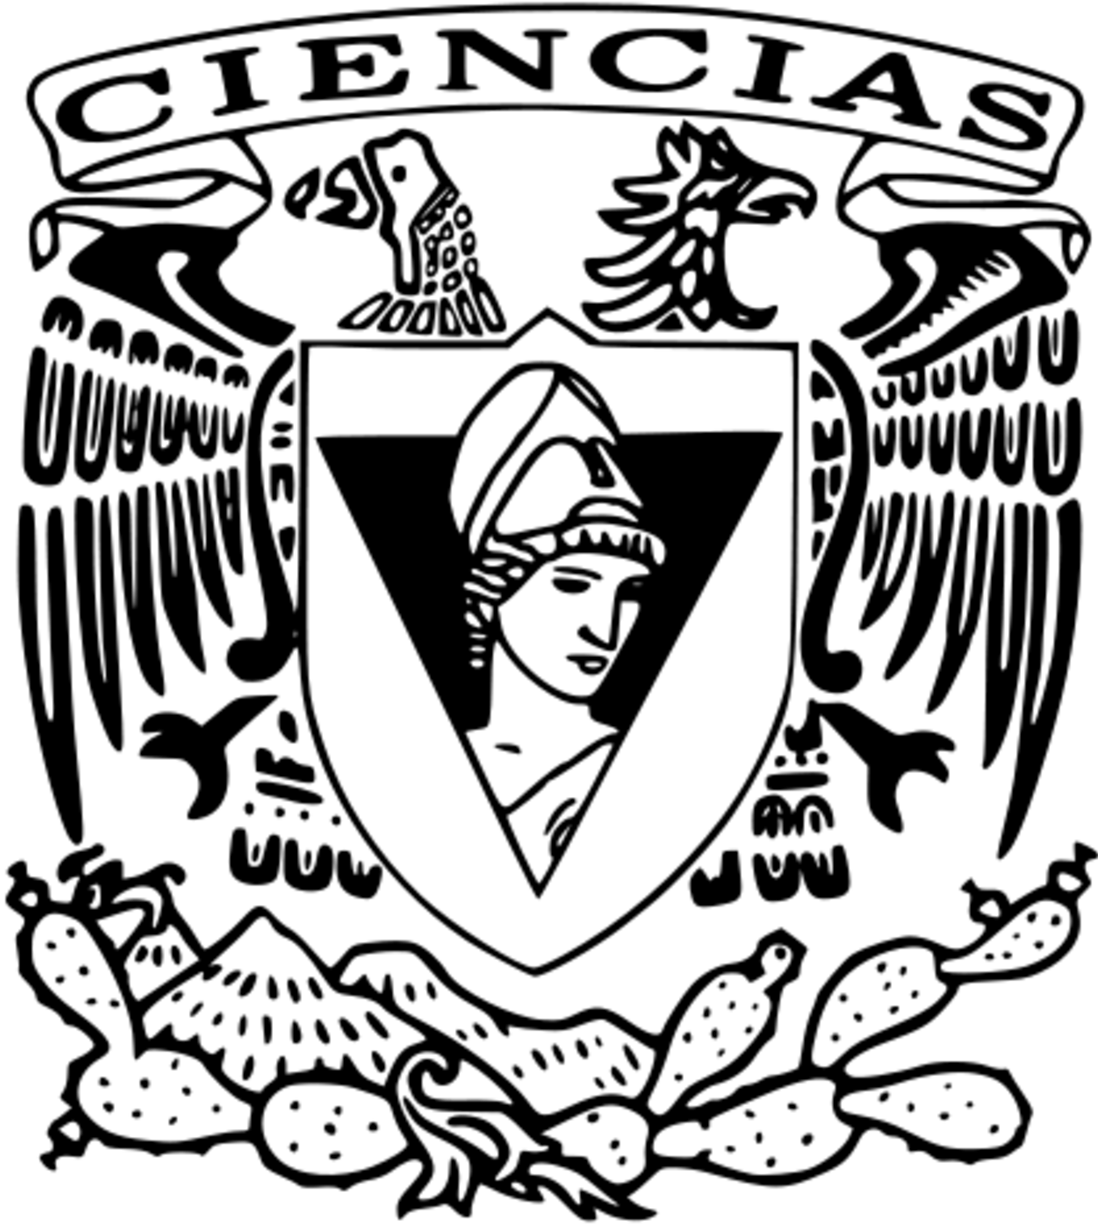
\includegraphics[height=4.0cm]{resources/Logo_FC.png}
		\end{center}
	\end{minipage}
	\begin{minipage}[c][0.81\textheight][t]{0.75\textwidth}
		\begin{center}
			\vspace{1cm}
			
			{\large\scshape Fundamentos de Bases de Datos - 7094}\\[.2in]
			
			\vspace{2cm}            
			
			\textsc{\LARGE \textbf{T}\hspace{1cm}\textbf{A}\hspace{1cm}\textbf{R}\hspace{1cm}\textbf{E}\hspace{1cm}\textbf{A}\hspace{1cm}\hspace{1cm}\textbf{4}}\\[2cm]
			\textsc{\Large{Equipo:}\normalsize \\
                \vspace{.3cm}
				\textbf{Del Monte Ortega Maryam Michelle - 320083527 \\
                \vspace{.2cm}
				\href{https://github.com/JuanSosaCiencias}{\textcolor{blue}{Sosa Romo Juan Mario - 320051926}} \\
                \vspace{.2cm}
				Castillo Hernández Antonio - 320017438 \\
                \vspace{.2cm}
                Erik Eduardo Gómez López - 320258211 \\
                \vspace{.2cm}
                Julio César Islas Espino - 320340594}}\\[0.5cm]     
			
			\textsc{{Fecha de entrega: \\ \textbf{10 de Octubre de 2024}}}\\[0.5cm]        
			
			\textsc{{Profesor: \\ \textbf{M. en I. Gerardo Avilés Rosas}}}\\[0.5cm]  
			
			\textsc{Ayudantes: \\ \textbf{Luis Enrique García Gómez \\ Kevin Jair Torres Valencia \\ Ricardo Badillo Macías \\ Rocío Aylin Huerta González
			} }
			
			
			\vspace{0.5cm}
		\end{center}
	\end{minipage}
\end{titlepage}


	
	\begin{center}
		\section*{\LARGE{Practica 6}}
	\end{center}
    % Preguntas  
    \begin{center}
        \LARGE{\textbf{Preguntas}}\\
    \end{center}
    \normalsize
    \begin{enumerate}%[label=\alph*.]
        \item \begin{center}
    \textbf{Menciona 5 diferencias sentre almacenar la informacion utilizando un sistema de archivos o almacenarla utilizando una BDD.}
\end{center}

\begin{enumerate}
    \item \textbf{Estructura de Datos:} Los sistemas de archivos son simples colecciones de archivos sin relación entre ellos, mientras que             las bases de datos organizan los datos de manera estructurada y con relaciones lógicas.
    \item \textbf{Redundancia:} La redundancia de datos es alta en los sistemas de archivos, ya que los mismos datos pueden aparecer en                 múltiples lugares. En las bases de datos, la redundancia se minimiza mediante normalización.
    \item \textbf{Consistencia de Datos:} Los sistemas de archivos tienen problemas de inconsistencia cuando los datos se modifican en                 varios archivos. En las bases de datos, las actualizaciones se reflejan de manera consistente en todas las instancias de los datos.
    \item \textbf{Seguridad:} Los sistemas de archivos suelen ofrecer menos seguridad, mientras que las bases de datos incluyen medidas de             seguridad avanzadas como control de acceso y encriptación. 
    \item \textbf{Copia de Seguridad y recuperación:} Los sistemas de archivos no cuentan con mecanismos automatizados de respaldo y                     recuperación, mientras que las bases de datos generalmente incluyen estas funciones para proteger la información.\\
\end{enumerate}
\cite{guru99, sooluciona}

\vspace{.5cm}



        \item \textbf{¿Qué ventajas y desventajas encuentras al trabajar con un Sistema de Bases de Datos
considerando que se planea implantar este sistema en una empresa de telemarketing?} \\

En primera instancia tenemos que reconocer que el telemarketing es una técnica publicitaria que es utilizada por las empresas para contactar con potenciales clientes y hablarles acerca de sus productos o servicios . \\

Hay muchas empresas a lo largo del mundo que hacen de esta estrategia su principal manera de operar, catalogándose en mayor o menor medida como empresas de telemarketing y si bien cada empresa decide como gestionar sus recursos para así poder llegar a su publico objetivo, el telemarketing cuenta con una serie de ventajas y desventajas enumeradas de la siguiente manera las cuales pueden hacer que una empresa se decante por este sistema o no: \\


\begin{table}[h!]
    \centering
    \begin{tabular}{|p{6cm}||p{6cm}|}
        \hline
        \textcolor{blue}{\textbf{Ventajas}} & \textcolor{Red}{\textbf{Desventajas}} \\ \hline 
        Se tiene un trato mas directo con los potenciales clientes & Si se utiliza de manera inadecuada puede afectar negativamente a la reputación de la empresa \\ \hline
        Permite entrar en contacto con un gran número de clientes en poco tiempo & En algunos países existen ciertas restricciones para esta clase de técnicas \\ \hline 
        Permite ofrecer una gran cantidad de información sobre el producto o servicio en cuestión  & Requiere una inversión en formar a los agentes y que estos sigan las buenas practicas de la empresa \\ \hline
        Se puede llamar a cualquier parte del mundo, lo cual asegura que nuestra empresa pueda darse a conocer en otras fronteras & La tasa de conversión es baja\\ \hline
    \end{tabular}
    \caption{Ventajas y desventajas de un Sistema de Telemarketing \cite{boada_cyberclick_2023}} 
\end{table}

Así mismo el telemarketing puede utilizarse de distintas maneras y estas varían de acuerdo a la campaña y objetivos de la empresa. Pero volviendo al punto principal de la pregunta, algunas de las posibles ventajas y desventajas de implemmentar un sistema de base de datos en alguna empresa de telemarketing podrian ser las siguientes:\\


\begin{table}[h!]
    \centering
    \begin{tabular}{|p{6cm}||p{6cm}|}
        \hline
        \textcolor{green}{\textbf{Ventajas}} & \textcolor{purple}{\textbf{Desventajas}} \\ \hline
        Organización y gestión eficiente de datos & Altos costos de implementación y mantenimiento continuo. \\ \hline
        Generación de análisis detallados e historial de datos. & Trabajo extra para integración con sistemas existentes y necesidad de capacitación del personal. \\ \hline
         Automatiza las tareas repetitivas y hay una reducción de errores manuales. & Riesgo de interrupciones por fallos del sistema y necesidad de ajustes por actualizaciones. \\ \hline
        Tiene la capacidad para manejar más datos y mas personalización según necesidades específicas. &  Riesgos de seguridad y necesidad de cumplir con normativas de privacidad. \\ \hline
        Existe un control de acceso a datos sensibles y así como también un respaldo de datos. & Existen riesgos por parte de entradas de datos incorrectos y problemas de duplicados. \\ \hline
    \end{tabular}
    \caption{Ventajas y desventajas de un Sistema de BD en una empresa de telemarketing}
    \cite{adSalsa_2024}
\end{table}

    \end{enumerate}
    \newpage
    
\printbibliography
  
\end{document}